%----------------------------------------------------------------------------------------
%	PACKAGES AND OTHER DOCUMENT CONFIGURATIONS
%----------------------------------------------------------------------------------------

\documentclass[11pt,a4paper]{article}

\usepackage[utf8]{inputenc}
\usepackage[dutch]{babel}
\usepackage{amsmath}
\usepackage{amsfonts}
\usepackage{amssymb}
\usepackage[left=2cm,right=2cm,top=2cm,bottom=2cm]{geometry}
\usepackage{graphicx}
\usepackage{float}
\graphicspath{{figures/}}
\usepackage{todonotes}
\usepackage{url}
\usepackage{subcaption}
%----------------------------------------------------------------------------------------
%	CONFIGURATION OF CODE LISTINGS
%----------------------------------------------------------------------------------------

\usepackage{listings}
\usepackage{color}
 
\definecolor{codegreen}{rgb}{0,0.6,0}
\definecolor{codegray}{rgb}{0.5,0.5,0.5}
\definecolor{codepurple}{rgb}{0.58,0,0.82}
\definecolor{backcolour}{rgb}{0.95,0.95,0.92}
 
\lstdefinestyle{mystyle}{
    backgroundcolor=\color{backcolour},   
    commentstyle=\color{codegreen},
    keywordstyle=\color{magenta},
    numberstyle=\tiny\color{codegray},
    stringstyle=\color{codepurple},
    basicstyle=\footnotesize,
    breakatwhitespace=false,         
    breaklines=true,                 
    captionpos=b,                    
    keepspaces=true,                 
    numbers=left,                    
    numbersep=5pt,                  
    showspaces=false,                
    showstringspaces=false,
    showtabs=false,                  
    tabsize=2
}
 
\lstset{style=mystyle}

\begin{document}

\begin{titlepage}

\newcommand{\HRule}{\rule{\linewidth}{0.5mm}} % Defines a new command for the horizontal lines, change thickness here

\center % Center everything on the page
 
%----------------------------------------------------------------------------------------
%	HEADING SECTIONS
%----------------------------------------------------------------------------------------

\textsc{\textsc{\LARGE KU Leuven}}\\[1.5cm] % Name of your university/college
\textsc{\Large Modellering \& Simulatie}\\[0.5cm] % Major heading such as course name
\textsc{\large Verslag practicum 2}\\[0.5cm] % Minor heading such as course title

%----------------------------------------------------------------------------------------
%	TITLE SECTION
%----------------------------------------------------------------------------------------

\HRule \\[0.4cm]
{ \huge \bfseries Bedrijfskasstroomsimulaties}\\[0.4cm] % Title of your document
\HRule \\[1.5cm]
 
%----------------------------------------------------------------------------------------
%	AUTHOR SECTION
%----------------------------------------------------------------------------------------

\begin{minipage}{0.4\textwidth}
\begin{flushleft} \large
\emph{Auteur:}\\
Ward \textsc{Schodts} % Your name
\end{flushleft}
\end{minipage}
~
\begin{minipage}{0.4\textwidth}
\begin{flushright} \large
\emph{Begeleiders:} \\
Prof. Dr. Ir. Ronald \textsc{Cools} \\ % Supervisor's Name
Prof. Dr. Ir. Wim \textsc{Michiels} \\ % Supervisor's Name
Prof. Dr. Ir. Dirk \textsc{Nuyens} \\ % Supervisor's Name
Dr. Ir. Nick \textsc{Vannieuwenhoven} \\ % Supervisor's Name
\end{flushright}
\end{minipage}\\[4cm]

% If you don't want a supervisor, uncomment the two lines below and remove the section above
%\Large \emph{Author:}\\
%John \textsc{Smith}\\[3cm] % Your name

%----------------------------------------------------------------------------------------
%	DATE SECTION
%----------------------------------------------------------------------------------------

{\large \today}\\[3cm] % Date, change the \today to a set date if you want to be precise

%----------------------------------------------------------------------------------------
%	LOGO SECTION
%----------------------------------------------------------------------------------------

\includegraphics[scale=0.15]{sedes}\\[1cm] % Include a department/university logo - this will require the graphicx package
 
%----------------------------------------------------------------------------------------

\vfill % Fill the rest of the page with whitespace

\end{titlepage}

\section*{Opdracht 1}

\lstinputlisting[language=Matlab, caption=Opdracht 1]{../r0381767_simulatePrice.m}

\section*{Opdracht 2}
De prijs gebruikt voor de opdracht is die van vrijdag 18 december 2015: \$$34.73$.

\begin{figure}[H]
\centering
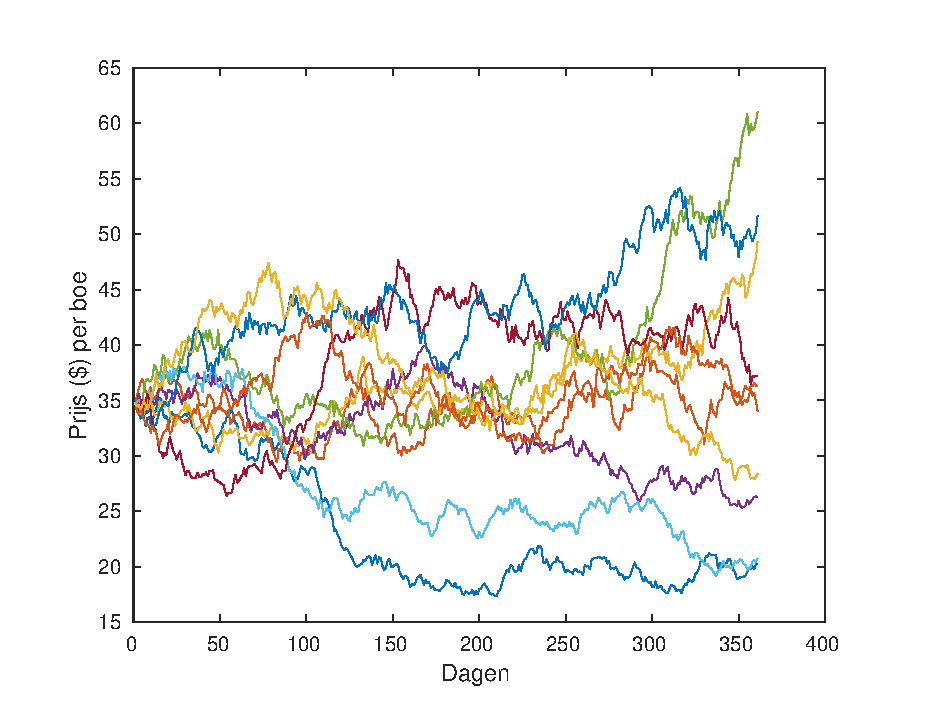
\includegraphics[scale=0.75]{opdracht2}
\caption{10 simulaties voor 360 dagen}
\end{figure}

\noindent
Het verloop van de olieprijzen getoond in bovenstaande figuur zien er realistisch uit als ze vergeleken worden met de olieprijs gedurende een jaar op de website van Bloomberg.

\lstinputlisting[language=Matlab, caption=Opdracht 2, firstline=1, lastline=9]{../opdrachten.m}

\section*{Opdracht 3}

\lstinputlisting[language=Matlab, caption=Opdracht 3]{../r0381767_averageOilPrices.m}

\section*{Opdracht 4}

\begin{figure}[H]
\centering
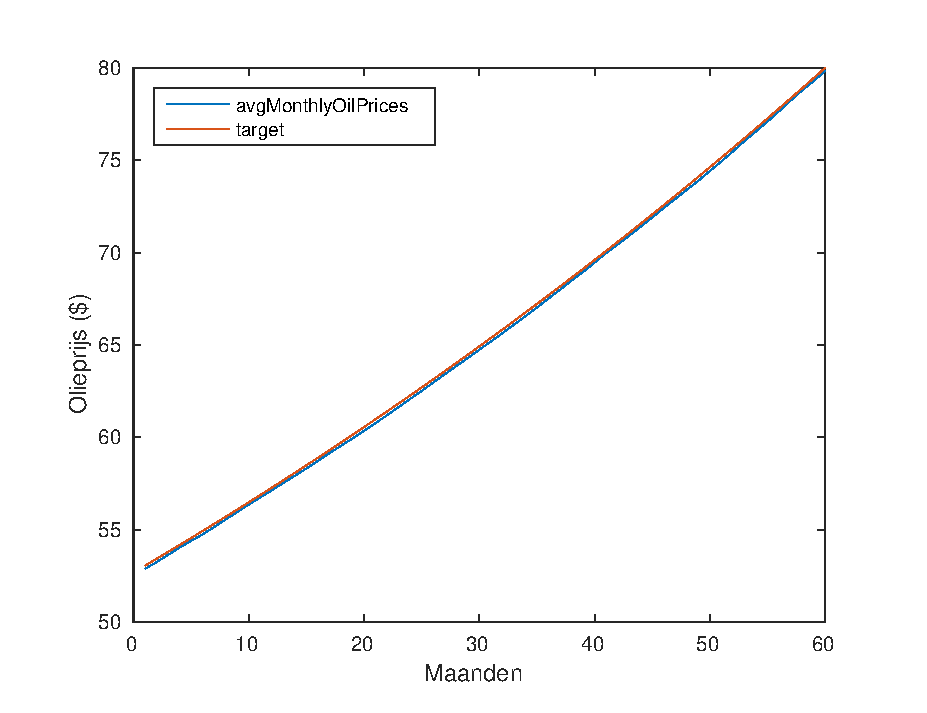
\includegraphics[scale=0.75]{opdracht4}
\caption{10 simulaties voor 360 dagen}
\end{figure}

\lstinputlisting[language=Matlab, caption=Opdracht 4, firstline=17, lastline=34]{../opdrachten.m}

\section*{Opdracht 5}
Het upstreamsegment van Shell realiseert een positieve winst vanaf een olieprijs van: \$$45.0412$.
\lstinputlisting[language=Matlab, caption=Opdracht 5, firstline=35, lastline=42]{../opdrachten.m}

\section*{Opdracht 6}

\lstinputlisting[language=Matlab, caption=Opdracht 6]{../r0381767_upstreamEarnings.m}

\section*{Opdracht 7}
De prijs gebruikt voor de opdracht is die van vrijdag 18 december 2015: \$$34.73$.
Shell realiseert dan een operationele nettowinst van het upstreamsegment van \$$-420000000$.
\lstinputlisting[language=Matlab, caption=Opdracht 7, firstline=43, lastline=46]{../opdrachten.m}

\section*{Opdracht 8}

\lstinputlisting[language=Matlab, caption=Opdracht 8]{../r0381767_downstreamEarnings.m}

\section*{Opdracht 9}
De prijs gebruikt voor de opdracht is die van vrijdag 18 december 2015: \$$34.73$.
Shell realiseert dan een operationele nettowinst van het downstreamsegment van \$$1710300000$.

\lstinputlisting[language=Matlab, caption=Opdracht 9, firstline=47, lastline=49]{../opdrachten.m}

\section*{Opdracht 10}

\lstinputlisting[language=Matlab, caption=Opdracht 10]{../r0381767_dividendExpense.m}

\section*{Opdracht 11}

\lstinputlisting[language=Matlab, caption=Opdracht 11]{../r0381767_capexExpense.m}

\section*{Opdracht 12}
De totale uitstaande schuld van Shell op 1 januarie 2015 bedraagt: \$$44.8898$ miljard.
\lstinputlisting[language=Matlab, caption=Opdracht 12, firstline=51, lastline=56]{../opdrachten.m}

\section*{Opdracht 13}

\lstinputlisting[language=Matlab, caption=Opdracht 13]{../r0381767_interestExpense.m}

\section*{Opdracht 14}
De maximale hoeveelheid interest (\$$0.1952$ miljard) wordt terugbetaald in december 2015. De totale hoeveelheid interest bedraagt \$$11.4416$ miljard en de totale hoeveelheid van de hoofdsommen \$$33.4482$ miljard. 
Alle schuld van obligaties is terugbetaalt na de 360 maanden.
\lstinputlisting[language=Matlab, caption=Opdracht 14, firstline=57, lastline=67]{../opdrachten.m}

\section*{Opdracht 15}
\begin{figure}[H]
\centering
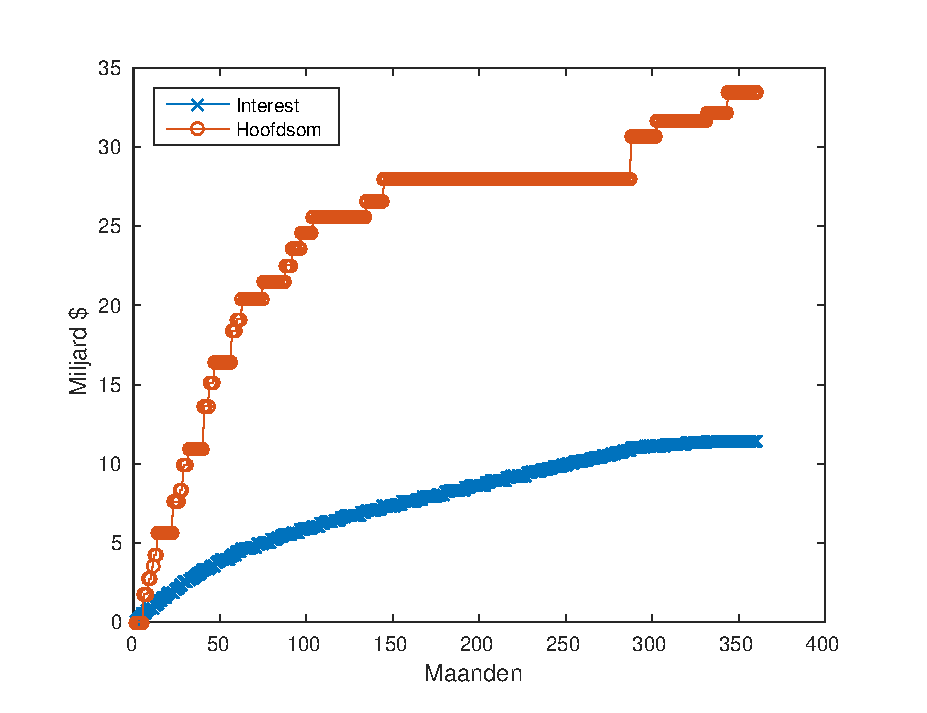
\includegraphics[scale=0.75]{opdracht15}
\caption{Interestlasten en hoofdsom voor 360 maanden}
\end{figure}

\lstinputlisting[language=Matlab, caption=Opdracht 15, firstline=68, lastline=76]{../opdrachten.m}
\section*{Opdracht 16}

\lstinputlisting[language=Matlab, caption=Opdracht 16]{../r0381767_cashFlow.m}

\section*{Opdracht 17}
\begin{figure}[H]
\centering
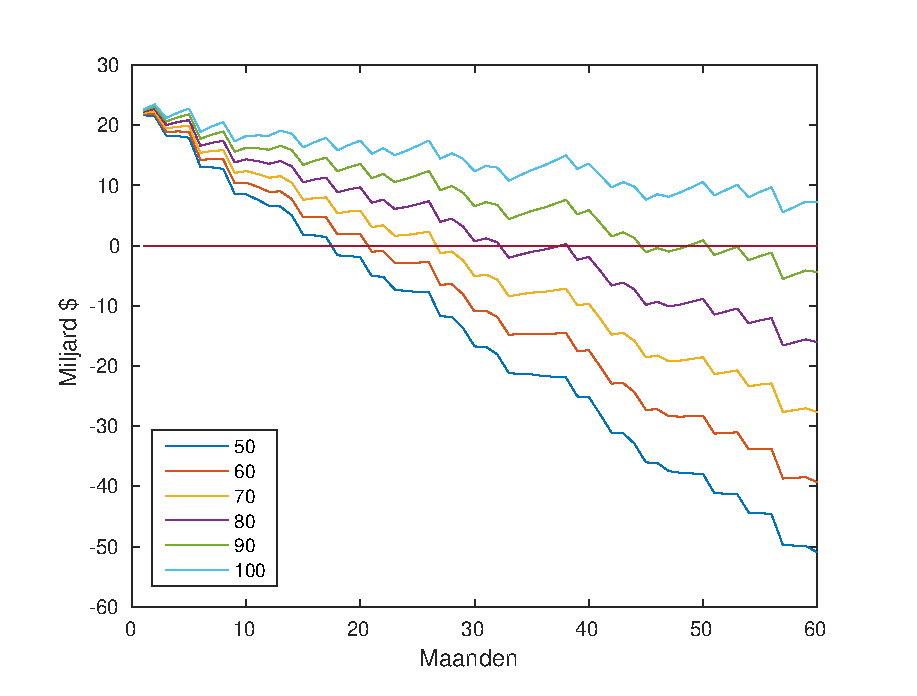
\includegraphics[scale=0.75]{opdracht17}
\caption{Simulatie met vaste olieprijs en zonder herfinanciering}
\end{figure}

\lstinputlisting[language=Matlab, caption=Opdracht 17, firstline=77, lastline=99]{../opdrachten.m}

\section*{Opdracht 18}
\begin{table}[H]
\centering
\begin{tabular}{c|c|c}
Prijs & Maand & Jaar\\
\hline
\$50 & maart & 2016\\
\$60 & juni & 2016\\
\$70 & november & 2016\\
\$80 & maart & 2017\\
\$90 & september & 2017\\
\$100 & september & 2018\\
\end{tabular}
\end{table}
De code om de data te vinden zit mee in opdracht 17, zie dus listing 17.
\section*{Opdracht 19}

\lstinputlisting[language=Matlab, caption=Opdracht 19]{../r0381767_cashFlowWithRefinancing.m}

\section*{Opdracht 20}

\begin{figure}[H]
\centering
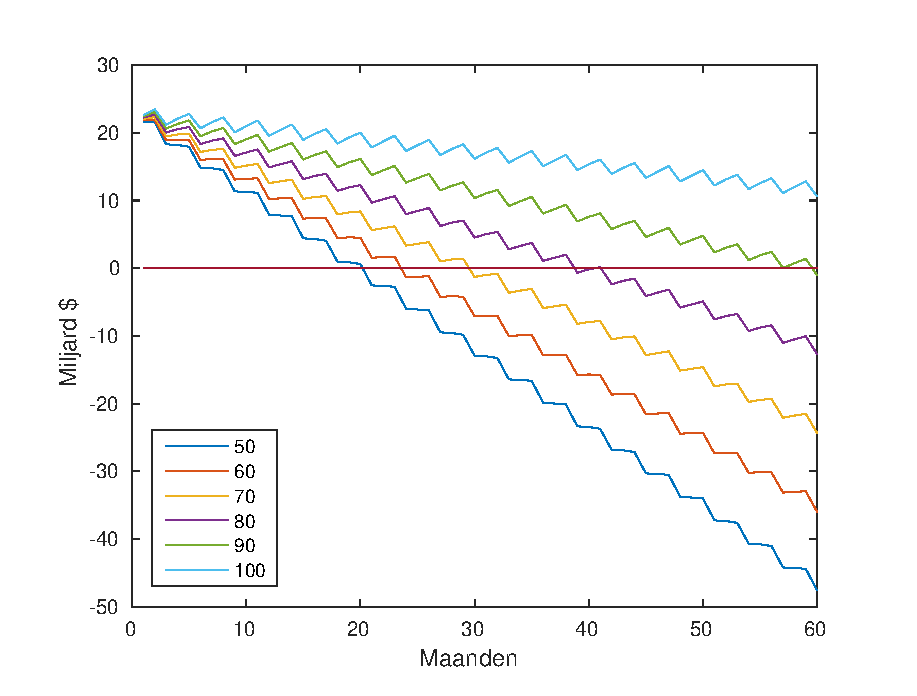
\includegraphics[scale=0.75]{opdracht20}
\caption{Simulatie met vaste olieprijs en met herfinanciering}
\end{figure}

\lstinputlisting[language=Matlab, caption=Opdracht 20, firstline=100, lastline=122]{../opdrachten.m}

\section*{Opdracht 21}

\begin{table}[H]
\centering
\begin{tabular}{c|c|c}
Prijs & Maand & Jaar\\
\hline
\$50 & september & 2016\\
\$60 & december & 2016\\
\$70 & juni & 2017\\
\$80 & maart & 2018\\
\$90 & december & 2019\\
\$100 & ? & ?\\
\end{tabular}
\end{table}

\section*{Opdracht 22}

\begin{figure}[H]
\centering
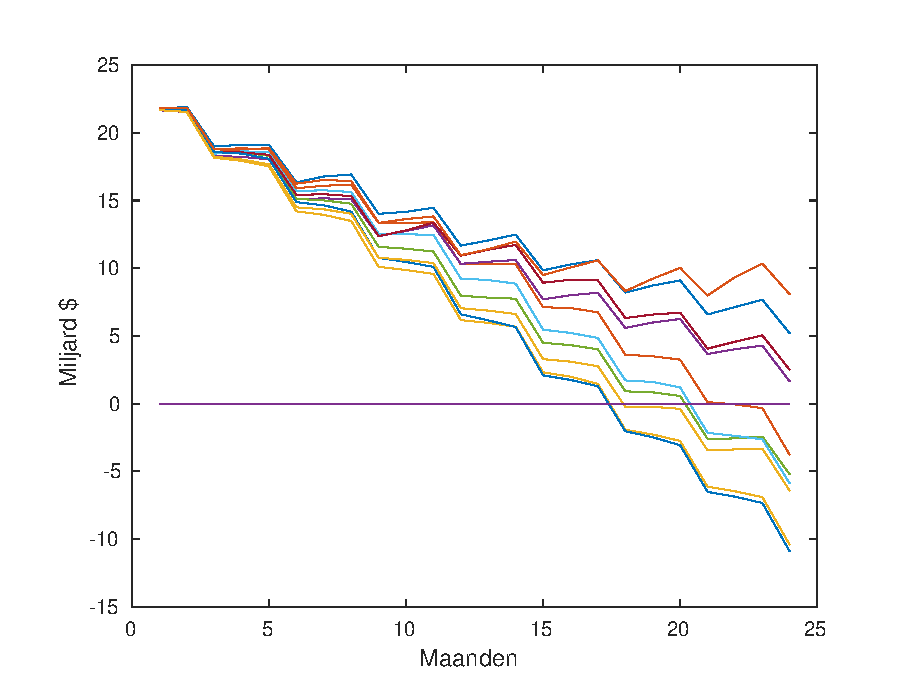
\includegraphics[scale=0.75]{opdracht22}
\caption{Simulatie met gesimuleerde olieprijs en met herfinanciering}
\end{figure}
Bij deze simulatie gaat Shell in 6 gevallen failliet.

\lstinputlisting[language=Matlab, caption=Opdracht 22, firstline=123, lastline=135]{../opdrachten.m}

\section*{Opdracht 23}

De kans bedraagt 69.55\%.

\lstinputlisting[language=Matlab, caption=Opdracht 23, firstline=136, lastline=146]{../opdrachten.m}

\section*{Opdracht 24}

Oplossen opdrachten: 12u.\\
Verslag maken: 8u.

\section*{Opdracht 25}

Ik denk niet dat de simulaties die wij hebben gemaakt echt een nut hebben. Ze zijn te simplistisch om veel waarde aan te hechten. 
Het lijkt me niet realistisch dat een oliebedrijf als Shell failliet zou gaan, ondanks de dalende olieprijs. 

\section*{Opdracht 26}
Dit practicum was gemakkelijker als het vorige. Soms heb ik wel het gevoel dat er enkel geïmplementeerd moet worden, ik zou graag wat meer achtergrond krijgen hoe men bijvoorbeeld tot het model (vergelijking 1 in de opgave) komt.
De economische terminologie is voldoende duidelijk.
Zelf ben ik tegen bedrijven zoals Shell en Total, ik zou liever vraagstukken zien voor bedrijven met een beter imago.

\end{document}